\begin{exercise}
      {ID-3b39ef2bf4c9a24096d1db3196d4dde89213f980}
      {Grundstück}
  \ifproblem\problem
    \begin{minipage}[c]{0.38\textwidth}
      \centering
      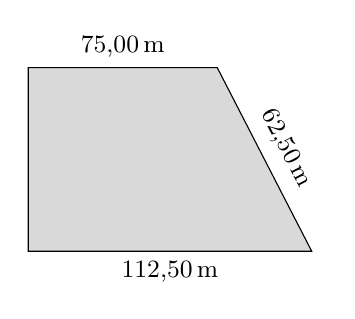
\begin{tikzpicture}[scale=0.32]
        \coordinate (A) at ( 0.00, 0.00);
        \coordinate (B) at (11.25, 0.00);
        \coordinate (C) at ( 7.50, 7.29);
        \coordinate (D) at ( 0.00, 7.29);
        \draw[fill=black!15!white] (A) -- (B) -- (C) -- (D) -- cycle;
        \path (A) -- node[below] {{\small112,50\,m}} (B);
        \path (C) -- node[above] {{\small75,00\,m}} (D);
        \path (B) -- node[shift=(27.5:3mm), rotate=-62.5] {{\small62,50\,m}} (C);
      \end{tikzpicture}
    \end{minipage}\hfill
    \begin{minipage}[c]{0.6\textwidth}
      Ein trapezförmiges Grundstück soll verkauft werden. Der Besitzer verlangt
      \eur{32} für einen Quadratmeter. Wie teuer ist das gesamte Grundstück?
    \end{minipage}
  \fi
  %\ifoutline\outline
  %\fi
  %\ifoutcome\outcome
  %\fi
\end{exercise}
